% NOTE: docs/paper/preserve-dont-resolve.md is the CANONICAL source (decided 2026-07-02).
% This .tex is a ported build target. Do not hand-edit content here; edit the markdown and
% re-port. Build: latexmk -xelatex preserve-dont-resolve.tex
\documentclass[11pt]{article}

% ---------- Packages ----------
\usepackage[margin=1in]{geometry}
\usepackage{fontspec}
\setmonofont{Menlo}
\usepackage{microtype}
\setlength{\emergencystretch}{3em}
\sloppy
\usepackage{booktabs}
\usepackage{array}
\usepackage{graphicx}
\usepackage{amsmath}
\usepackage{amssymb}
\usepackage{amsthm}
\usepackage{tikz}
\usetikzlibrary{arrows.meta,positioning,shapes.geometric,decorations.pathreplacing}
\usepackage[T1]{fontenc}
\usepackage[english]{babel}
\usepackage{csquotes}
\usepackage[authoryear,round]{natbib}
\usepackage{enumitem}
\usepackage{fvextra}
\usepackage{xcolor}
\usepackage{hyperref}
\hypersetup{hidelinks}

% ---------- Theorem-like environment ----------
\newtheorem{invariant}{Invariant}

% ---------- Verbatim prompt style ----------
\DefineVerbatimEnvironment{promptverb}{Verbatim}{fontsize=\small,frame=single,xleftmargin=2mm,xrightmargin=2mm,breaklines=true,breaksymbolleft={}}

% ---------- Title ----------
\title{Preserve, Don't Resolve: Non-Fabrication and Provenance as the Evaluation Axis for Agent Memory}
\author{Mihir Wagle \\ Independent Researcher \\ \texttt{mihir.wagle@gmail.com}}
\date{Draft of 2026-07-02}

\begin{document}

\maketitle

\begin{abstract}
Agent memory systems are benchmarked on accuracy: return the current value of a fact after
a long, noisy history. We argue this is the wrong axis once a trivial recency baseline
already wins it, and that the right axis is two guarantees a consolidating memory
sacrifices: non-fabrication (never asserting a current value that was not established) and
provenance (which source governs, and what it superseded). We call the design that holds
them preserve-not-resolve, and its keystone invariant: a tension may never masquerade as a
supersession. We evaluate daftari, a memory whose no-mint guarantee is structural rather
than model-dependent, against consolidation baselines across two contrasting regimes on
the recency axis: formal contract amendment chains, where recency is accuracy-sufficient,
and Wikipedia consensus records, where recency returns a stale value on 33/33 supersession
traps. The separating axis is the same in both regimes. Forced to maintain a single
current value, a three-model panel collapses genuine, editor-certified tensions into
supersessions in 17 of 18 trials, while daftari mints zero values and manufactures zero
false conflicts in either regime; the one deployed consolidator we ran never registers the
correction at all on 26 of 33 traps. The honest limit: a capable, abstain-prompted LLM
approximates non-fabrication on average, but only by failing to detect real supersessions,
and without the structural guarantee an auditor needs.
\end{abstract}

\section{Introduction}
\label{sec:introduction}

A memory system for an autonomous agent is usually benchmarked the way a database is: pose
a question whose answer changed over a long history, and score whether the system returns
the \emph{current} value. This framing makes recall the figure of merit and ``staying current''
the hard problem, which in turn motivates \textbf{consolidation}, periodically rewriting the
store into a compact, current summary (the ``sleep'' or ``dreaming'' pass of recent agent-
memory systems).

We make two claims against this framing. First, the consumer of the memory is an \emph{agent},
not a human reader, and what the agent needs is not a pre-computed answer but structure
it can reason over: what is current, what that rests on, and what is contested. Second,
once a system \emph{resolves} a history into a single current value, it has discarded exactly
that structure, and the discarding is not free, because the resolution can be \emph{wrong} in
two ways a recall metric does not see: it can \textbf{fabricate} a value that was never
established, and it can \textbf{erase provenance} (which source governs, what it superseded,
whether the matter was ever settled). We call the design that refuses to resolve
\textbf{preserve-not-resolve}, and its load-bearing invariant, which we will call the
\textbf{keystone} throughout (Invariant~\ref{inv:keystone}):

\begin{invariant}
\label{inv:keystone}
A tension may never masquerade as a supersession.
\end{invariant}

A \emph{supersession} is a settled replacement (B is now current, it replaced A on the merits).
A \emph{tension} is an unresolved disagreement (A and B are both live; neither has won). A
consolidating memory that must store one current value has no representation for the
second, so it records the first: it lets a tension wear the clothes of a supersession.
The agent downstream then reads a confident ``current value'' where the truth is ``contested,
status quo by default.''

This paper evaluates preserve-not-resolve against consolidation across two corpora chosen
to differ on the one axis a skeptic cares about: \emph{whether recency already solves
accuracy}. Contracts are the \textbf{recency-works regime}: a trivial baseline is
accuracy-sufficient, so accuracy cannot be the contribution, which forces the honest
question of what a memory owes you when recency is already right. Wikipedia consensus
records are the \textbf{recency-fails regime}: recency genuinely returns stale values, and the
corpus contains real, editor-certified tensions. Our contribution is the \textbf{measured
invariance}: the separating axis is the same in both regimes, with a precise account of
where the guarantee is structural and where it softens to a model-dependent behavior.

We describe the system under test (\S\ref{sec:system}), the two-regime design (\S\ref{sec:regimes}), the results in each
regime (\S\ref{sec:contracts}--\S\ref{sec:wikipedia}), the direct measurement of the keystone (\S\ref{sec:keystone}), the synthesis (\S\ref{sec:synthesis}), an
adversarial self-assessment with explicit kill conditions (\S\ref{sec:honest}), related work (\S\ref{sec:related}), and
limitations (\S\ref{sec:limitations}).

\section{The system under test: a preserve-not-resolve memory}
\label{sec:system}

We evaluate \textbf{daftari}, a Model Context Protocol (MCP) server that exposes a curated
markdown vault to agents. Its design choices are the ones that matter for this paper:

\begin{itemize}
\item \textbf{Markdown + YAML frontmatter} is the substrate; the frontmatter is the metadata layer.
  Every fact is a document an agent (or human) can read directly.
\item \textbf{Git is the version layer.} Every write auto-commits; nothing is destroyed. This zeroes
  \emph{irreversibility} as a variable, a property we exploit in \S\ref{sec:honest} and that a companion study,
  in preparation, builds on.
\item \textbf{Supersession is a pointer, not a value.} When a document is superseded, daftari records
  an edge \texttt{superseded\_by → <successor path>}; it never mints a new consolidated value. A
  query that asks for the current value follows the pointer; it does not read a rewritten
  summary.
\item \textbf{Tensions are first-class and are not auto-resolved.} A contested relationship is logged
  as a tension (\texttt{vault\_tension\_log}, \texttt{vault\_edge\_contest}); the system surfaces it and
  leaves resolution to a human. There is, by design, no automatic pass that converts a
  tension into a supersession.
\item \textbf{The query path calls no LLM.} Retrieval and current-source resolution are deterministic
  (lexical + vector ranking, pointer-following). The consolidation loop (named ``cortex'' by
  analogy to sleep-time memory consolidation), which is advisory and out of scope for this
  paper's measurements, emits \emph{edges}, never prose.
\end{itemize}

The single structural fact that drives every result below: daftari has no operation that
mints a current value from a contested history. Its no-mint property is therefore a
guarantee by construction, not a behavior we hope a model exhibits. The systems contribution
is that a memory built this way is still \emph{useful}: it answers ``what is current'' by
following pointers, while never being forced to manufacture an answer it does not have.

\begin{figure}[t]
\centering
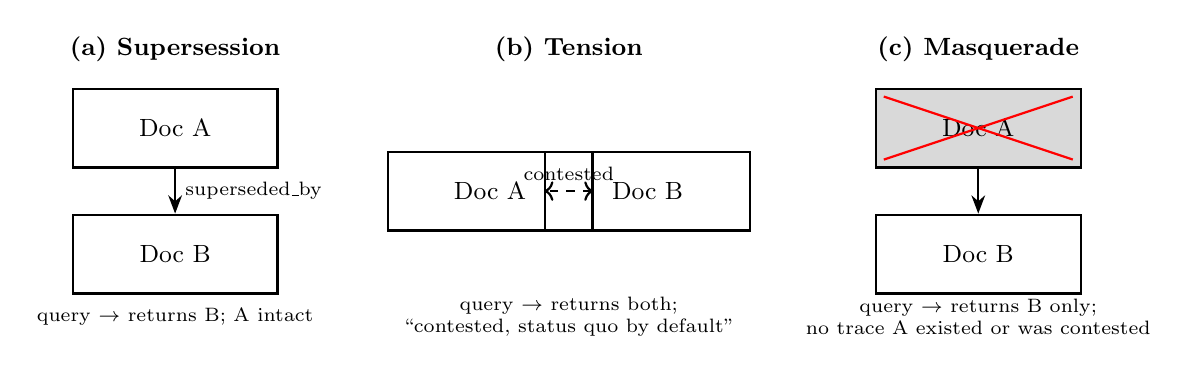
\begin{tikzpicture}[
  box/.style={draw, thick, minimum width=2.6cm, minimum height=1cm, align=center, font=\small},
  supbox/.style={box, fill=gray!8},
  arr/.style={-Stealth, thick},
  panel/.style={font=\bfseries\small}
]
% Panel (a): Supersession
\node[panel] at (0,2.0) {(a) Supersession};
\node[box] (a1) at (0,1.0) {Doc A};
\node[box] (b1) at (0,-0.6) {Doc B};
\draw[arr] (a1) -- node[right,font=\scriptsize]{superseded\_by} (b1);
\node[font=\scriptsize] at (0,-1.4) {query $\rightarrow$ returns B; A intact};

% Panel (b): Tension
\node[panel] at (5.0,2.0) {(b) Tension};
\node[box] (a2) at (4.0,0.2) {Doc A};
\node[box] (b2) at (6.0,0.2) {Doc B};
\draw[arr, <->, dashed] (a2) -- node[above,font=\scriptsize]{contested} (b2);
\node[font=\scriptsize,align=center] at (5.0,-1.4) {query $\rightarrow$ returns both;\\ ``contested, status quo by default''};

% Panel (c): The masquerade
\node[panel] at (10.2,2.0) {(c) Masquerade};
\node[box,fill=gray!30] (a3) at (10.2,1.0) {Doc A};
\node[box] (b3) at (10.2,-0.6) {Doc B};
\draw[arr] (a3) -- (b3);
\draw[thick,red] (9.0,0.6) -- (11.4,1.4);
\draw[thick,red] (9.0,1.4) -- (11.4,0.6);
\node[font=\scriptsize,align=center] at (10.2,-1.4) {query $\rightarrow$ returns B only;\\ no trace A existed or was contested};
\end{tikzpicture}
\caption{The three-panel supersession/tension/masquerade mechanism. (a) Supersession: document A
with a \texttt{superseded\_by} pointer to document B; a query follows the pointer and returns B,
with A intact behind it. (b) Tension: A and B joined by a contested edge; a query returns both
positions plus ``contested, status quo by default.'' (c) The masquerade: a one-slot
consolidating store where B has overwritten A (A shown crossed out); the query returns B with no
trace that A existed or that the matter was contested. Panel (c) is what the keystone forbids.}
\label{fig:mechanism}
\end{figure}

\textbf{What the agent does with this.} The payoff of preserving structure is a decision the agent
could not otherwise make (Figure~\ref{fig:mechanism}). Consider an agent asked to act on a contested fact: to execute a
clause whose governing value is disputed, or apply a policy two stakeholders still disagree
on. Against a consolidating memory it receives a single confident current value and acts; the
tension is invisible, so the wrong action is indistinguishable from the right one. Against
daftari the same query returns the \emph{structure}: a \texttt{superseded\_by} pointer where the matter is
settled, or a logged tension where it is not. On the tension the agent reads \emph{contested,
status quo by default}, and can take the branch a minted value would have hidden: abstain from
the irreversible action, surface both positions, escalate to a human. We do not evaluate this
downstream behavior (that is a claim about agents, not memory); we note only that the structure
daftari preserves is the input such behavior requires, and that a minted value destroys it
before the agent ever sees the choice.

\section{Two regimes, one axis}
\label{sec:regimes}

The competitor we measure against is a \textbf{consolidating / value-minting memory}: a system
whose job is to maintain a single current-state record, of which the deterministic
``most-recent-mention'' baseline and an LLM-consolidation step are two instances. The question
is when, and how, such a system fails in a way preserve-not-resolve does not.

We select two corpora as \textbf{contrasting regimes on the recency axis}:

\begin{itemize}
\item \textbf{Regime one: formal contracts (recency works).} Amendment chains where a trivial
  most-recent-mention baseline returns the correct current value. If a difference shows here,
  it is \emph{not} about accuracy.
\item \textbf{Regime two: Wikipedia consensus records (recency fails).} Human decision records where
  recency returns stale values, and where genuine unresolved tensions exist.
\end{itemize}

A word on what this design is and is not. It is tempting to call the pair a control and a
treatment, and earlier drafts did; we avoid that vocabulary because it belongs to randomized
designs, and nothing here is randomized or assigned. What the pair actually is is a
\emph{most-different-cases} design, a severe test: two regimes chosen to be maximally unlike on
the one axis a skeptic cares about, with the claim that the separating axis is the same in
both. The regimes also differ on axes we did not choose: genre (legal drafting vs.
encyclopedic dispute), ground-truth source (deterministic chain resolution vs.
editor-maintained decision records), task shape (clause reconstruction vs. directional
supersession verdicts), and unit of analysis (clauses vs. edit pairs). We therefore do not
claim recency-resolvability is isolated as a manipulated variable; no two corpora could
deliver that. The invariance argument survives these confounds because the claim is
existential per regime, not a corpus-level effect estimate: in each regime, read on its own
terms, the minting failure and the provenance failure appear, and the no-mint property
holds. A confound would have to explain both appearances away independently, in corpora
that share almost nothing else.

Two corpora that differ on the axis a skeptic cares about is a \emph{design}, not a sample size;
adding a third corpus of the same shape would answer ``does it replicate?'', which is not the
question. The contribution is the invariance of the separating axis across the two
opposite regimes (\S\ref{sec:synthesis}).

\begin{figure}[t]
\centering
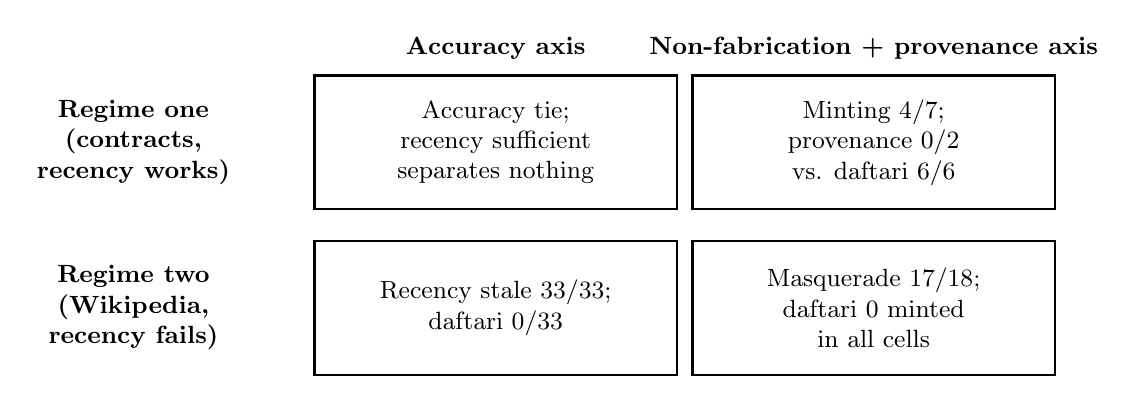
\begin{tikzpicture}[
  cell/.style={draw, thick, minimum width=4.6cm, minimum height=1.7cm, align=center, font=\small},
  rowlabel/.style={font=\bfseries\small, align=center},
  collabel/.style={font=\bfseries\small, align=center}
]
\node[collabel] at (2.6,3.6) {Accuracy axis};
\node[collabel] at (7.4,3.6) {Non-fabrication + provenance axis};

\node[rowlabel] at (-2.0,2.4) {Regime one\\(contracts,\\recency works)};
\node[cell] (r1c1) at (2.6,2.4) {Accuracy tie;\\ recency sufficient\\ separates nothing};
\node[cell] (r1c2) at (7.4,2.4) {Minting 4/7;\\ provenance 0/2\\ vs. daftari 6/6};

\node[rowlabel] at (-2.0,0.3) {Regime two\\(Wikipedia,\\recency fails)};
\node[cell] (r2c1) at (2.6,0.3) {Recency stale 33/33;\\ daftari 0/33};
\node[cell] (r2c2) at (7.4,0.3) {Masquerade 17/18;\\ daftari 0 minted\\ in all cells};
\end{tikzpicture}
\caption{The invariance argument as a $2\times2$ grid. Rows: regime one (recency works,
contracts) and regime two (recency fails, Wikipedia). Columns: the accuracy axis and the
non-fabrication + provenance axis. Cells carry the \S\ref{sec:synthesis} numbers: accuracy tie / stale 33/33;
minting 4/7 and 17/18; provenance 0/2 vs.\ 6/6; daftari 0 minted in all cells. The left column
separates nothing, the right column separates everything, in both rows.}
\label{fig:regimes}
\end{figure}

\textbf{Experimental setup.} All foil, judge, and second-rater LLM calls in \S\ref{sec:contracts}--\S\ref{sec:keystone} are routed
through OpenRouter, never called directly against a vendor API, so a single client and a
single cost/logging path cover every model in the panel. The panel: \texttt{anthropic/claude-
haiku-4.5}, \texttt{z-ai/glm-4.6}, and \texttt{openai/gpt-4o} as the foil/consolidation-baseline models;
\texttt{google/gemini-2.5-flash} as the cross-family second-rater and blind judge, chosen to be
independent of every foil family and of daftari's own client (Anthropic-only). We did not
pin dated API snapshot IDs; OpenRouter model slugs (as shown above) are what the runners
recorded, and access ran across late June 2026 (2026-06-27 through 2026-06-29, per the
run dates in the released results notes). Every run in \S\ref{sec:contracts}--\S\ref{sec:keystone} is a single run at temperature
0; we did not average over repeated samples, and we say so again at each point a number is
reported so a reader never has to infer it. Approximate per-experiment cost, where the
running note recorded one: CB4 (Wikipedia derivation + foil panel) \textasciitilde\$1, CB5 (contradiction
detector, full-passage and span-level) \textasciitilde\$0.4, CB6 (the keystone panel, \S\ref{sec:keystone}) \textasciitilde\$2, the
Wikipedia Arm B pilot \textasciitilde\$1; the contracts-side forced-Arm-B and provenance runs (\S\ref{sec:contracts}) did not
record a cost figure in the running notes, so none is claimed for them beyond ``small,
n=6-7 calls per model per condition.''

\textbf{Attrition accounting.} The Wikipedia corpus starts from 37 consensus-citing-revert
instances; 33 are scorable (single-hunk, cleanly diffable) and 4 are excluded as multi-hunk
(a revert touching several passages at once, which the scoring pipeline cannot align to one
stale/governing pair), excluded for that structural reason and not because they were
inconvenient. daftari's Arm C localizes and returns the governing value on 16 of the 33 (\S\ref{sec:wikipedia});
this is stated in full in \S\ref{sec:wikipedia} and is not repeated here. Separately, the first attempt at the
CB4 foil-panel run returned output the parser could not read across all 33 pairs: the
acquirer had omitted the schema embedding daftari's own derivation classifier depends on
(\texttt{completeJson}), so the model's replies did not match the expected shape. The run was fixed
to faithfully reproduce that schema embedding and re-run; the numbers reported in \S\ref{sec:wikipedia} and \S\ref{sec:synthesis}
are from the corrected re-run, not the unparseable first attempt, and no data from the first
attempt is used anywhere in this paper.

\section{Regime one: contracts, where recency is accuracy-sufficient}
\label{sec:contracts}

\textbf{Corpus.} Real SEC EDGAR credit-agreement amendment chains (e.g., Natural Gas Services
Group), pulled deterministically, with a zero-LLM resolution pipeline that classifies each
amendment operation as recoverable (whole-clause/defined-term restate, delete, add) or
unrecoverable (partial edits, ``the last sentence of Section X is amended\ldots''). Contamination
is controlled by value-perturbation: a deterministic, seeded, type/magnitude-preserving
substitution of the measured value classes (durations, currency amounts, percentages), so
memorized contracts cannot be answered from priors. The substitution is seeded per chain and
carried across every document in a chain with one shared mapping, so a value that recurs
across the master agreement and its amendments is replaced identically everywhere, while a
value a later amendment changes maps to a different fake than the value it superseded; the
mapping is persisted alongside the corpus so ground truth is regenerable. We did not run a
collision check against real-world values external to the corpus; the assumption, not
independently verified, is that collision probability is negligible at this value-class
range. Procedure and collision-avoidance details beyond what is stated here are in the
released benchmark code.

\textbf{Accuracy is solved by a trivial baseline.} A stale-restatement probe over both real
chains found zero cases where a later document quotes a \emph{superseded} value as current;
the structural reason is incorporation-by-reference drafting (``terms have the meaning set
forth in the Credit Agreement, \emph{as amended}''), so recitals never quote stale values. Corpus-
wide, operative-amendment idioms outnumber the only stale-value-quoting idiom by \textgreater100:1.
On a clean real chain, most-recent-mention recency and daftari's chain-following resolution
\emph{tie} on accuracy. The formality that makes contract supersession explicit and labelable
is the same formality that makes it recency-resolvable, so accuracy cannot be the
contribution here. Good: it forces the question this paper is about.

\textbf{Non-fabrication (the partial-amendment subset).} Where a clause's current value is \emph{not
recoverable} from what was retrieved (partial amendments that edit a sub-part without
restating the whole), a value-minting baseline must still emit a value. Under the realistic
consolidation shape (a forced answer, no abstain), two cross-family foils (GPT-4o,
Gemini-2.5-flash) fabricate a governing value on 4/7 partial clauses each; daftari emits
0/7 by construction (it points to the governing source and flags the clause
unrecoverable). With an abstain option offered, the LLM baseline fabricates less (1/7), the
first appearance of a pattern we quantify in \S\ref{sec:keystone}. Both foils fabricated the \emph{same} 4 of the 7
clauses, and flagged the same 3 as unrecoverable: at n=7 this looks clause-driven (some
operative phrasings signal partiality more explicitly than others) rather than model-driven,
though n=7 is too small to separate the two cleanly; we treat the 4/7 and 1/7 figures as
existence demonstrations that forcing fabricates, not as precise rate estimates.

\textbf{Provenance (where LLMs actually fail).} Asked for the per-clause governing source and
supersession history, an LLM-over-raw-documents baseline reproduces provenance for \emph{clean}
clauses (history 5--6/6, governing 4/4) but mis-attributes governance on the \emph{partial}
clauses 0/2: it defaults to the last-touched amendment where the correct answer is the
master agreement, \emph{even when the resolution rule is stated in the prompt}. daftari's
deterministic resolution is 6/6. At n=2 this is an existence demonstration, not a rate:
what the result shows is that naive provenance \emph{can} fail exactly on the partial clauses,
even when told the rule, not what fraction of partial clauses it fails on. The qualitative
claim survives the small n: a consolidation architecture has no representation that
distinguishes a partial edit from a clean supersession, so it discards which source governs
by construction, independent of how often that shows up empirically at this sample size.

\textbf{Reading.} On contracts, daftari's value concentrates entirely on the unrecoverable/partial
subset, exactly where minting fabricates and naive provenance mis-attributes, while clean
clauses are recency-resolvable. Accuracy is not the axis; non-fabrication and provenance are.

\section{Regime two: Wikipedia consensus, where recency fails}
\label{sec:wikipedia}

\textbf{Corpus.} The \texttt{Talk:<Article>/Current consensus} subpages, human-maintained, dated
decision records for high-conflict articles, with explicit consensus-citing reverts in the
article's revision history. Ground truth is the editor-maintained consensus box, not an LLM
labeler, so the label side carries no LLM-contamination risk; alignment of a stale edit to
the governing decision is editor-provided (``rv per consensus \#N''). Memorization is addressed
two ways. First, a post-cutoff subset: of the 37 instances, 14 fall after the training
cutoff (2025--26), 12 are scorable, and the stream-recency baseline is stale on all 12; this
agrees with the full-corpus 33/33 and is a robustness check, not an independent sample.
Second, the foil-side text itself (the passages the minting and contradiction-detector
foils read) is largely pre-cutoff, unperturbed Wikipedia prose, a limitation we do not paper
over: to the extent a foil model recognizes the passage from training, that familiarity
should, if anything, help it recognize which value is current and abstain or answer
correctly, so the fabrication numbers we report are conservative, not inflated, with respect
to this exposure. Pre-cutoff value-perturbation, applied to the contracts corpus (\S\ref{sec:contracts}), was
not run on Wikipedia; we list it as a limitation (\S\ref{sec:limitations}).

\textbf{Recency fails; daftari never goes stale.} Across the 33 scorable supersession traps, a
stream-recency baseline (trusting the latest ingested edit; the streaming form of \S\ref{sec:contracts}'s
most-recent-mention foil, one foil family in both regimes) returns a stale value 33/33
before the governing edit and the correct value after (a fair foil); daftari's chain-
following resolution is never stale (0/33). The one-sided 95\% Clopper-Pearson lower bound
on 33/33 is approximately 0.91: even reading the result conservatively, recency fails on this
corpus at a rate no plausible sampling variation explains away. daftari's coverage on the same
33 pairs is partial, not complete: it localizes and returns the governing value on 16/33
(where the governing consensus item carries an inline marker daftari can resolve against) and
abstains on the rest rather than guess; on none of the 33 does it assert a stale value.

\textbf{Auto-acquisition is hard, by design, and the result reflects it.} We tested whether
daftari's \emph{actual} derivation classifier auto-acquires the stale$\leftrightarrow$governing relation: recall
1/33, because competing wordings are a \emph{tension}, not a load-bearing derivation, so the
classifier correctly declines and the system mints 0. A bespoke contradiction detector
(the ``right lens'') recovers little more: 2/33 over full passages, 4/33 when narrowed to the
changed span, because most of these disputes are \emph{framing/detail} differences (both
versions true), not logical contradictions, with false-positive 0/16 and 0 minted
throughout. The honest reading: these conflicts are largely \emph{not recoverable from text
alone}; the editor process surfaces them from edit/rule context. daftari's claim is
no-mint, not auto-acquisition.

\textbf{The minting foil fabricates, but how much is model-dependent.} Offered an abstain option
(NEITHER, available to all three models on the panel), a value-minting baseline asked for a
directional supersession verdict on the 49 stale/governing and cross-item pairs is
position-biased and fabricates: total fabrication F = 26/49 for a cheap model
(Haiku-4.5), 24/49 for GLM-4.6, but only 6/49 for GPT-4o, which takes the abstain it
is offered, returning ``neither'' on 25/33 real pairs. So the abstain-offered fabrication is
model-dependent (6--26/49), and capability does not predict aggressiveness: the most
capable model is the most restrained. This is the same softness as \S\ref{sec:contracts}'s abstain-offered 1/7.
On this corpus the forced condition (no abstain option) is measured only at n=6, in \S\ref{sec:keystone}; it is
\emph{not} the robust headline here, \S\ref{sec:keystone} is. All panel numbers above are a single run at
temperature 0; we did not average over repeated samples.

\textbf{A deployed consolidator, measured.} The foils above are prompt-level models of
consolidation; a fair objection is that a real consolidating memory's write path might behave
better, for instance by declining a bad update (a no-op). We ran one: Mem0's actual write path
(v2.0.11, default configuration, \texttt{openai/gpt-4o} via OpenRouter, temperature 0, a fresh store
per item) over the same corpus, ingesting the stale edit and then the governing decision for
each of the 33 traps, and both positions for each of the 6 tensions. The result is a \emph{third}
failure mode, neither fabrication nor clean overwrite: on 26/33 traps, ingesting the
governing correction added nothing to the store; the extraction step judged it redundant
against the stale memory already present, so the correction was silently never registered.
This is not graceful abstention: the store's current state remains the stale value with no
record that a correction arrived. (Notably, this version's default write path is additive
only; the ADD/UPDATE/DELETE loop described in the Mem0 paper is reachable only through
explicit API calls, and 78/78 ingests produced ADD.) On the 6 tensions both positions
survived in 5/6, but as a byproduct of the same additive-only behavior, not tension
awareness. The measured system is therefore not the better-abstaining consolidator the
objection imagines; where recency fails, it fails more quietly than the recency baseline,
because the correction never even enters the store. Single run; one system and version; we
state it as a bound on the objection, not a survey of consolidators.

\section{The keystone, measured}
\label{sec:keystone}

The keystone (Invariant~\ref{inv:keystone}), \emph{a tension may never masquerade as a supersession}, would
be empty if it held only ``by construction.'' We measure it directly.

\textbf{Genuine tensions, editor-certified.} A consensus item closed \textbf{``no consensus''} is a
genuine tension: the status quo holds \emph{by default}, not by superseding the alternative on the
merits. The editors label this verbatim (e.g., ``\ldots there is no consensus on specific wording,
but the status quo is X''; a Request for Comment (RfC), Wikipedia's formal
dispute-resolution process, closed ``status=No consensus''). We collected the six
currently-active such items across the three articles whose consensus box records
them (Donald Trump $\times$4, Joe Biden, COVID-19 pandemic; a survey of 12 candidate articles found
the box is a rare institution). For each, the two competing positions were distilled from
the linked RfC and gated by a second rater (``is this a genuine unresolved disagreement where
neither has won out?''), 6/6 validated. The second rater is \texttt{google/gemini-2.5-flash} via
OpenRouter: cross-family relative to both the foil panel (Haiku-4.5, GLM-4.6, GPT-4o) and the
daftari contradiction detector (Anthropic Haiku), blind to which item came from which source,
one run. Two follow-up checks then removed this gate's evidential weight, and we report
both. First, a negative control: fed 8 verifiably \emph{settled} supersessions (selected
mechanically from the 33 traps) under the identical prompt, in the same session in which it
re-passed the 6 tensions 6/6, the gate rejected only 2/8; it is a near-uniform approver.
Second, a human rating pass over the same pairs, with three settled controls embedded
blind (rater: the author, disclosed), broke the instrument in the opposite direction: the
rater read the same question as asking whether the two \emph{texts} substantively conflict, and
under that reading found genuine conflict in 0/6 tensions, the inverse of the LLM's
near-uniform yes. A question whose meaning flips between raters validates nothing, so the
gate carries no weight here. The human 0/6 is itself a datum, though: a human expert
reading the paired texts alone cannot see the tension, the human analogue of the
detector's 2--4/33 (\S\ref{sec:wikipedia}); the unresolvedness of these disputes is carried by the editorial
record, not the wording. The validation the gate was meant to provide was then re-run
properly: an independent, non-author rater, blind to provenance and to which items were
controls, judged the pairs meaningfully distinct 4/6 (the two exceptions are the two
closest near-paraphrase pairs) and fairly stated 4/6, and, asked whether the text
alone reveals the dispute's outcome with ``cannot tell'' explicitly legitimized, asserted a
winner on 6 of 9 answered items, choosing the first-presented position all six times
and scoring 1/3 (chance) on the settled controls. Outcomes are not recoverable from
these texts even when a rater asserts one, and a human offered an abstain option behaves
like the abstain-offered models: sometimes manufacturing a direction anyway, with position
bias. Accordingly, the \emph{unresolvedness} of the six tensions rests on the editor ``no
consensus'' closes themselves, which are the corpus's ground truth by construction and do
not pass through any gate or rater. Ground truth = \textbf{NEITHER supersedes}.

\textbf{Two conditions.} A consolidation memory whose architecture maintains a single current
value has no ``tension'' slot; we model this with the \textbf{forced} condition (the foil must pick a
direction). An LLM consolidation step that \emph{could} decline is modeled by the
\textbf{abstain-offered} condition.

\begin{table}[t]
\centering
\begin{tabular}{lccc}
\toprule
condition & Haiku-4.5 & GLM-4.6 & GPT-4o \\
\midrule
\textbf{Forced masquerade} (architectural) & 5/6 & 6/6 & 6/6 \\
Abstain-offered (LLM judgment) & 3/6 & 5/6 & 2/6 \\
\textbf{daftari} (structural) & 0/6 & 0/6 & 0/6 \\
\bottomrule
\end{tabular}
\caption{Forced-masquerade, abstain-offered, and daftari results on the six editor-certified
tensions. Cells count tensions collapsed into a supersession, of the 6 editor-certified
tensions. daftari's row is identical by construction for any model: no operation in its
write or query path can mint the directional verdict the foil rows count, so the 0/6 holds
independent of the model column (its contradiction detector, which runs on Haiku, is
measured separately below: 0/6 false conflicts manufactured).}
\label{tab:keystone}
\end{table}

\begin{itemize}
\item \textbf{Forced.} 17/18 across the panel: a memory that must emit one value collapses a genuine
  tension into a supersession, \emph{near model-independently} (GPT-4o masquerades 6/6 when it
  cannot abstain). The condition is not a sterile tautology: Haiku \emph{refused} once. The 18 forced trials are 6
  items times 3 models, and a model's verdicts are not independent draws across items, so we
  also report the item-clustered count: 6/6 items were masqueraded by at least 2 of the 3
  models (GLM-4.6 and GPT-4o both went 6/6, Haiku missed only one), a Wilson 95\% interval of
  roughly [0.61, 1.00] on that proportion. The trial-level 17/18 and the item-level 6/6 point
  the same direction; we report both because trials sharing an item are not independent
  evidence.
\item \textbf{daftari.} Mints 0/6 and manufactures 0/6 false conflicts: its contradiction detector
  flags the 3 genuinely oppositional items and correctly declines on the 3 framing disputes:
  it neither mints a supersession nor invents a contradiction; it preserves both positions.
\item \textbf{Abstain-offered.} Model-dependent (2/6--5/6): GLM-4.6 most aggressive, GPT-4o most
  restrained.
\end{itemize}

All panel numbers in this section are a single run at temperature 0. The forced condition
(17/18) is stable across the panel and near model-independent, so we read it as robust; the
abstain-offered condition is not: at temperature 0 it still shifts run-to-run, so the 2/6--5/6
range should be read as one sample of the model-dependent softness, not a precise estimate of
any model's abstention rate.

This is the keystone as an architectural fact, not a claim about model quality.

\section{Synthesis: the invariance}
\label{sec:synthesis}

Place the two regimes side by side (Table~\ref{tab:synthesis}):

\begin{table}[t]
\centering
\small
\begin{tabular}{p{3.1cm}p{5.4cm}p{5.4cm}}
\toprule
axis & Contracts (recency works) & Wikipedia (recency fails) \\
\midrule
Accuracy & recency sufficient ($>$100:1); tie & recency stale 33/33; daftari 0/33 \\
Minting fabricates & partial clauses: forced 4/7 (abstain-offered 1/7) & forced tensions 17/18; abstain-offered 6/49 to 26/49 across models \\
Provenance & LLM governing 0/2 on partials; daftari 6/6 & supersession pointer preserved; tension preserved \\
Deployed consolidator (Mem0 v2.0.11) & not run & correction silently unregistered 26/33; tensions kept 5/6 (additive-only) \\
Values minted by daftari & 0/7 partial clauses & 0/49 pairs + 0/6 tensions \\
\bottomrule
\end{tabular}
\caption{Synthesis of the two regimes on the accuracy axis and the non-fabrication +
provenance axis.}
\label{tab:synthesis}
\end{table}

\begin{center}
\begin{minipage}{0.9\textwidth}
\small
\emph{Note.} The Wikipedia minting cell mixes two datasets by design: 17/18 is over the 6 tension items
across the 3-model panel (\S\ref{sec:keystone}); the abstain-offered fabrication counts are over the 49
stale/governing and cross-item pairs (\S\ref{sec:wikipedia}).
\end{minipage}
\end{center}

The separating axis is the same in both regimes: non-fabrication and provenance, not
accuracy. And the system that holds it does so by construction. Where recency already
wins (contracts), accuracy cannot distinguish architectures, yet minting still fabricates on
partials and erases provenance. Where recency fails (Wikipedia), a memory that must resolve
collapses genuine tensions. In neither regime does daftari mint, for any model, with no
prompt engineering. That invariance, not any single fabrication number, is the
contribution.

A note on how to read daftari's own rows in this table and in \S\ref{sec:contracts}--\S\ref{sec:keystone}: because daftari's no-mint
behavior is by construction, every ``0'' is best read as an implementation-correctness
check, not a discovered rate. A bug in the chain-following or pointer-resolution code could
have produced a nonzero fabrication count on any of these corpora; it did not, on every corpus
we ran. The cleanest single number for this purpose is the false-positive control: 0/16
minted supersessions on the Wikipedia cross-item pairs that have no relation at all. That
daftari's design goal (never mint) and its measured behavior (0 everywhere) agree is evidence
the implementation matches the design, not evidence the design is hard to satisfy.

\section{Honest assessment and kill conditions}
\label{sec:honest}

We hold ourselves to an adversarial read.

\begin{itemize}
\item \textbf{The non-fabrication gap over a \emph{careful, abstain-prompted} LLM is small, and model-
  dependent.} Offered an abstain option, GPT-4o fabricates little (6/49 on Wikipedia, 1/7 on
  contracts). A reviewer will say: ``then just use GPT-4o and let it abstain.'' Three answers.
  (i) It abstains by failing to detect what is there: on the 33 real supersessions it
  returned ``neither'' 25/33; low fabrication bought with low recall is not a memory you trust.
  Put the two systems on the same 33 pairs directly: daftari answers 16 correct, 0 wrong
  (localizes where the governing item carries a marker, abstains on the rest, never asserts a
  stale value); GPT-4o, abstain-offered, answers 3 correct, 5 wrong-direction, 25
  abstained. daftari dominates on both axes at once, more correct answers and zero wrong
  ones, not a trade of recall for safety.
  (ii) daftari's guarantee is structural: it holds for any model, with no prompt
  engineering and no dependence on someone remembering to offer the abstain option; that is
  an auditability/worst-case property, not an average-case one. (iii) The real competitor
  is not ``a careful LLM you may ask to abstain'': a consolidation/accumulator memory emits
  a single current value (the forced condition, where the contrast is model-independent); a
  memory that abstains on every contested point is not doing the job daftari does (answer
  \emph{and} preserve the tension). The one deployed consolidator we ran (Mem0 v2.0.11, \S\ref{sec:wikipedia}) is
  not that careful abstainer either: its default write path silently failed to register the
  governing correction on 26/33 traps, leaving the stale value current with no trace.
\item \textbf{The components are not individually novel (\S\ref{sec:related}).} Bi-temporal supersession-without-
  deletion (Graphiti), unresolved-contradiction representation (ATMS), the supersession-vs-
  contradiction distinction (ElephantBroker), and supersession-preserving provenance (Roynard)
  all predate us. We claim the \emph{structural conjunction}, no-mint of a tension as a
  by-construction invariant, and the empirical measurement of \S\ref{sec:contracts}--\S\ref{sec:keystone}, not the constituent
  ideas. A reviewer who knows ElephantBroker will press hardest here; \S\ref{sec:related} carries the full
  defense (its split is LLM-extracted and confidence-decayed, exactly the model-dependence
  \S\ref{sec:keystone} measures).
\item \textbf{The keystone is measured at n=6.} Small, because the consensus box is a rare institution
  (3 articles). The structural guarantee is the backbone; the measurement is support. Scaling
  needs broad RfC-close harvesting, which loses the clean editor label.
\item \textbf{Tension pairs are distilled, then gated, and the gate did not survive its own audit.}
  The status-quo side is grounded in the box; the alternative is distilled from the RfC by
  the author (a judgment step). We had leaned on the second-rater gate (6/6, \S\ref{sec:keystone}) to shore
  this up; a negative-control run (gate rejects only 2/8 settled supersessions) and a human
  rating pass (the rater read the same question as textual conflict and answered 0/6, the
  inverse of the LLM) together invalidate the instrument, and we assign it no weight. What
  carries unresolvedness is the editor ``no consensus'' close, which never passes through a
  gate. The distillation itself was then validated by an independent, non-author rater
  (\S\ref{sec:keystone}): 4/6 pairs meaningfully distinct (the two exceptions are the near-paraphrase
  pairs), 4/6 fairly stated. The two fairness objections both name the author-distilled
  \emph{alternative} wording (the Accords and gaffes pairs), which we disclose as distillation
  defects rather than average away; the keystone counts are unchanged if those two items
  are dropped (forced masquerade 11/12 on the remaining four).
\item \textbf{Auto-acquisition on Wikipedia is low (1--4/33).} We claim no-mint, not auto-acquisition.
\item \textbf{The consolidation loop is described, not powered.} This paper makes no variance/quality
  claim about the loop; that is a companion study, in preparation.
\end{itemize}

\textbf{Single kill condition, with thresholds.} daftari has no niche if any consolidation
baseline, run on the released fixtures, achieves all four of the following at once:
(i) fabrication at most 1/49 on the Wikipedia pairs and at most 1/7 on the contract
partials (daftari's 0, within one miss); (ii) masquerade at most 1/6 on the tension items,
abstain permitted or not, its choice; (iii) governing-source attribution at least 5/6 on
contracts, including both partial clauses; and (iv) correct-answer coverage at least 16/33
on the Wikipedia traps, daftari's own coverage, so that (i) and (ii) are not bought with
blanket abstention. Measured so far, none does: the careful abstainer loses recall (3
correct, 25 abstained, of 33); the aggressive models fabricate (up to 26/49); none
reproduces partial-clause provenance (0/2); the forced minter masquerades 17/18; and the
one deployed consolidator we ran never registers the correction on 26/33. The condition is
prospective: we commit to running submitted baselines on the released fixtures, and the
strongest untested candidates (an actual Graphiti pipeline; a refusal-tuned model in the
Trust-Align family) are named in \S\ref{sec:related} rather than presumed to fail.

\section{Related work}
\label{sec:related}

The individual components of preserve-not-resolve are not novel, and we cite the prior
art rather than claim them; the contribution is their \emph{structural conjunction} on a specific
substrate, plus the empirical measurement of \S\ref{sec:contracts}--\S\ref{sec:keystone}. Several of the closest systems are 2026
preprints with no citation track record yet; every claim we attribute to one is grounded in
its primary text, not secondary coverage.

\textbf{The consolidation / accumulation pole.} The dominant frame for agent long-term memory is
consolidation, periodically rewriting memory toward a compact current state. Mem0
\citep{chhikara2025mem0} dynamically extracts and consolidates via ADD/UPDATE/DELETE operations that
overwrite prior entries (though in the shipped version we measured, v2.0.11, the default
write path is additive only and the update/delete operations are reachable only via explicit
API calls; \S\ref{sec:wikipedia}); A-MEM \citep{xu2025amem} performs ``memory evolution,'' mutating existing
memories in place; MemGPT/Letta \citep{packer2023memgpt} self-edits hierarchical memory blocks,
resolving a changed fact by overwriting it in place via a \texttt{working\_context.replace(\ldots)}
function call (the paper's own identifier; the Letta implementation names the corresponding
operation \texttt{core\_memory\_replace}); and Cognee
is a multi-store knowledge-graph memory layer whose enrichment pass (\texttt{memify}) updates and
prunes nodes, with explicit \texttt{delete}/\texttt{prune} operations (mechanism per its documentation;
\citep{markovic2025cognee} is a tuning/evaluation study of the framework). A recent 2026 survey
\citep{du2026survey} names ``continual consolidation'' and ``learned forgetting'' as open frontiers and
treats contradiction handling as a write-path engineering concern, not a first-class
invariant. Generative Agents \citep{park2023generative} is the
important exception on the preservation axis: its reflections are an \emph{additive} layer over a
retained observation stream, prior art for ``preserve raw, layer inference on top,'' though it
makes no supersession or non-fabrication claim.

\textbf{Two preservation axes, often conflated.} ``Preserving structure'' splits into two distinct
properties, and the prior art sits on different ones:

\emph{Supersession-preservation}: keep the \emph{old} fact as history, but resolve which is current.
Zep/Graphiti \citep{rasmussen2025zep} is the strongest instance: a bi-temporal graph (each edge carries
both the time a fact held in the world and the time it was recorded) that \emph{invalidates}
(not deletes) an edge on contradiction, setting the old edge's \texttt{t\_invalid} to the new edge's
\texttt{t\_valid} and retaining it as queryable history, but it always resolves, ``consistently
prioritizes new information when determining edge invalidation,'' yielding a single current
state per relationship. Roynard's ``Knowledge Layer'' \citep{roynard2026knowledgelayer} similarly records
supersession as a relationship and preserves both claims append-only with explicit
provenance, but it has no first-class unresolved state: supersession, evidence-gated, is its
only preservation-with-linkage mechanism (it resolves). SmartVector \citep{xu2026smartvector} makes the pattern explicit: it
preserves every superseded vector (an \texttt{ARCHIVED} state with \texttt{supersedes}/\texttt{superseded\_by}
edges, ``nothing deleted'') yet resolves every contradiction by a recency / source-authority /
feedback majority vote: preserve the past, vote away the present. That is the move our
keystone forbids. daftari sits on this axis too, and we claim no novelty for keeping the
superseded fact. Notably, Graphiti's recency-prioritized resolution is the
\emph{foil} behavior of \S\ref{sec:wikipedia}: on our recency-fails corpus the governing value is not the latest edit, so
a recency-resolving memory goes stale exactly as the recency baseline does (stated as
positioning; we did not run Graphiti).

\emph{Tension-preservation}: hold \emph{two still-live} claims open, unresolved, and never let one
quietly become current. This is the keystone axis, and it has prior art too. The classical
deep precedent is the assumption-based truth-maintenance system (ATMS) \citep{dekleer1986atms}:
contradictory derivations coexist across assumption-environments via consistent labels and
recorded ``nogoods,'' never collapsing to one belief set. In agent memory, ElephantBroker
\citep{lupascu2026elephantbroker} is the sharpest: it emits a \emph{contradiction edge} (both facts retain confidence)
distinct from a supersession edge, directly our distinction. So representing a tension is
not our novelty either. What no system makes it is a \emph{structural, by-construction}
property (see below).

\textbf{Why the tension-preservers fall short of a structural guarantee.} ElephantBroker, the
sharpest case, represents the tension/supersession distinction but does not \emph{guarantee}
no-mint: (i) the classification is made by an LLM extractor, \emph{model-dependent}, exactly the
dependence \S\ref{sec:keystone} measures; (ii) it does not preserve a tension neutrally: the contradiction edge
carries a retrieval-scoring penalty and the supersession path decays the old fact's
confidence; (iii) its consolidation engine canonicalizes near-duplicates and archives
low-confidence facts (an accumulation move); and (iv) its only \emph{architecture-enforced}
guarantees concern safety/contamination, not the minting of values. So the closest competitor
\emph{confirms} the gap: representing a tension is not the same as a by-construction invariant that
one can never become a supersession. Two other recent systems frame the contrast. TOKI
\citep{wang2026toki} formalizes contradiction \emph{resolution} as a bitemporal operator algebra, the
opposite choice: resolve, with theory, rather than preserve. And classical TMS (ATMS) achieves
its no-collapse property \emph{structurally} (nogoods are pre-compiled so a label can never contain
an inconsistent environment), but over logical assumption-sets, not over a human-readable,
agent-consumed memory substrate.

\textbf{Non-fabrication and provenance are behavioral, not structural, in prior work.} Faithfulness
in RAG is achieved by model alignment, not architecture: Trust-Align \citep{song2024trustalign} improves
correct refusal via preference tuning with no by-construction guarantee, and ``Correctness is
not Faithfulness'' \citep{wallat2024correctness} shows models post-rationalize (up to 57\% of citations unfaithful
in their experiment). Provenance exists but targets a different relation: Portable Agent Memory
\citep{ravindran2026portable} provides a Merkle-DAG of derivation lineage (tamper-evidence), not provenance over
what-supersedes-what; AIS \citep{rashkin2021ais} is an attribution \emph{measurement} framework, not a
guarantee. The inverse-substrate pole writes memory \emph{into the model} rather than an
external store: Cartridges \citep{eyuboglu2025cartridges} distills a corpus offline into a trainable KV-cache
(key/value vectors trained by back-propagation; 38.6$\times$ less memory and 26.4$\times$ higher throughput
than in-context learning), productized as Engram (2026). Such memory is opaque, non-versioned,
and carries no supersession or provenance representation, the inverse substrate choice to a
human-readable, git-versioned store. It optimizes for token-cost, not supersession, so the
contrast is one of substrate and aim, not a head-to-head on our axis.

\textbf{A reproducible accumulation-corpus benchmark, and the limit of measuring one corpus.}
data-olympus \citep{dataolympus2026} is the nearest peer on substrate: a governance-grade knowledge
base of markdown files with YAML frontmatter kept in git (no database, no proprietary schema,
the substrate choice we defend in \S\ref{sec:system}), paired with a deterministically reproducible
retrieval benchmark of 250 generated concepts and 500 queries spanning lifecycle-status,
lifecycle-graph, curated-trigger, and loosely-phrased semantic categories. Its published
numbers are an honest ground truth for what a governed store with an explicit status field
achieves on the accumulation half: staleness 0.000 on lifecycle-graph queries where a BM25
baseline scores 1.000 (it never serves a superseded rule), recall 1.000 on lifecycle-status
and on curated triggers, a 0.000 out-of-scope false-positive rate under abstention, and the
keyword-retrieval failure mode published rather than buried (0.036 recall on loosely phrased
queries that share almost no words with the authored rule, where the authors note every
keyword method does poorly and vector retrieval has the edge). We take these figures from the
project's benchmark and did not independently reproduce them. The two-corpus thesis does not
compete with this result; it holds that the result measures a strict subset of what a memory
substrate must. The staleness-and-supersede axis these numbers characterize lives entirely in
the accumulation corpus. The tension axis, two live documents contradicting without
adjudication, lives in the generative corpus, and no accumulation-only benchmark can surface
it, because a supersede chain has already collapsed the boundary case into a linear order
before any query is scored. The measurement is right; the frame is one corpus too narrow. That
data-olympus reaches these numbers on the same markdown-in-git substrate we adopt sharpens
rather than blunts the point: the separating variable is not the store but whether the
evaluation admits an unresolved state at all.

\textbf{The augmentation, measured.} The claim that no accumulation-only benchmark can surface the
tension axis is testable, so we tested it. Starting from data-olympus's own corpus (regenerated
bit-for-bit at its pinned release), we add a documented, regenerable \emph{feud} stratum: pairs of
co-active documents contradicting on one topic with no \texttt{superseded\_by} link and no recency
ordering between them, the boundary case a supersede chain cannot represent. To keep the case
non-trivial we author one side in the query's vocabulary and the other in a divergent framing (a
second team's language for the same decision), so ordinary retrieval surfaces the first and
buries the second; whether it does is measured, not assumed (15 of 25 topics bury the divergent
side under a 250-concept bed, the other 10 co-retrieve). An agent, under an identical prompt and
tool budget across arms, then answers and emits a structured evidence-state (\texttt{settled}
$\mid$ \texttt{contested} $\mid$ \texttt{unknown}) scored deterministically into
\{surface, pick, fabricate\}. On the buried topics, a supersede-chain arm (daftari with its
tension index withheld, the closest in-system stand-in for an accumulation store's read path)
surfaces the contradiction on 0.08 of trials; the tension-graph arm surfaces it on 0.42--0.46
(two-proportion $z$ of 6.5--7.0, $p < 10^{-10}$), pooled over three neutral models
(\texttt{gpt-5.4-mini}, \texttt{gemini-2.5-flash}, \texttt{gpt-5-mini}) at three repetitions. The
mechanism is the one the frame predicts: the tension edge is an id-level, lexical-independent
link, so it reaches the side retrieval could not; the supersede chain has no such object to
return. Two honesty bounds. First, the win is confined to the recall-limited regime: on the 10
co-retrieved topics every arm surfaces at 0.9--1.0, because a capable model surfaces a
contradiction it can already see, so the defensible claim is not ``an accumulation store cannot
surface a tension'' but ``it cannot surface one its retrieval buries,'' the realistic case at
scale. Second, the result replicates on daftari's own hybrid (BM25 + embedding) retrieval rather
than a stand-in ranker (the embedding signal did not rescue the buried side, burial held at 15 of
25), and inline surfacing is the robust delivery while a dedicated look-up tool helps only models
that reliably invoke it. This is a supplementary measurement on a synthetic augmentation, not a
load-bearing claim of the two-corpus thesis (which rests on
\S\ref{sec:contracts}--\S\ref{sec:keystone}); it is included because it converts the ``one corpus
too narrow'' argument from assertion to demonstration on the peer's own substrate.

\textbf{The gap this paper fills} (narrowed to be reviewer-defensible):
\begin{itemize}
\item \textbf{A structural, by-construction no-mint invariant \emph{in an agent-memory system}.} Classical
  TMS (ATMS) has a structural no-collapse guarantee, but over logical assumption-sets in a
  reasoning engine, not a persistent, natural-language, agent-consumed memory. Among
  \emph{agent-memory} systems, none makes no-mint architectural; the closest, ElephantBroker,
  falls short in the ways detailed above. Our contribution is porting the TMS no-collapse
  property \emph{to the agent-memory substrate as a by-construction invariant}.
\item \textbf{The empirical two-corpus invariance.} No prior system is evaluated for non-fabrication +
  provenance across a regime where recency works and a regime where it fails.
\item \textbf{Provenance over supersession.} Existing provenance is lineage/tamper-evidence (Portable
  Agent Memory) or source attribution (Roynard); provenance over \emph{what governs and what it
  superseded} is thinner prior art.
\item \textbf{The substrate.} Almost no cited system targets a human-readable, git-versioned, agent-consumed
  markdown vault (data-olympus is the exception, and shares it; our distinction from it is the
  two-corpus frame, not the store): the surveyed systems store memory in databases, opaque trainable tensors,
  or knowledge graphs, and a competitor has publicly argued markdown is \emph{not} agent memory
  \citep{zep2026markdown} because plain files lack a structured query surface. We take the point and
  invert it: in daftari the query surface \emph{is} a graph-and-vector index (\S\ref{sec:system}), but a derived,
  rebuildable one, while provenance is served by the files, where every superseded value
  survives as a git object an auditor can read \emph{without trusting the system that wrote it}.
  The property the critique calls a limitation is precisely the property an auditability
  guarantee needs.
\end{itemize}

\section{Limitations and future work}
\label{sec:limitations}

\begin{itemize}
\item \textbf{A genuine-tension corpus at scale} (beyond n=6) would move the keystone from ``measured
  on a rare institution'' to ``powered'', the natural next acquisition.
\item \textbf{The comprehension-load ablation} (does bounding how much inferred structure the
  consolidation loop may write, its budget of trusted derivations, reduce retrieval-quality
  variance in a domain where git has zeroed irreversibility?) is a companion study, in
  preparation; it needs a derivation-rich corpus and a variance harness, both absent here.
\item \textbf{Stronger-model and forced-condition coverage on contracts} (the forced-minting
  condition on contracts is n=7) would tighten \S\ref{sec:contracts} the way \S\ref{sec:keystone}'s panel tightened the keystone.
\item \textbf{Pre-cutoff value-perturbation was not run on the Wikipedia corpus} (\S\ref{sec:wikipedia}). It is applied on
  contracts (\S\ref{sec:contracts}), where it defeats verbatim training recall by construction. On Wikipedia the
  foils read largely pre-cutoff, unperturbed text; we argue this makes the reported fabrication
  conservative (training familiarity should help a foil abstain or answer correctly, not
  fabricate), but a perturbed or fully post-cutoff Wikipedia arm would close the gap directly.
\item \textbf{As-of-date querying is not first-class.} Because every write auto-commits, the vault's
  transaction-time history (what a document said at any past moment) is preserved losslessly and
  is fully auditable, which already separates it from an overwrite-in-place file store. It is
  not, however, queryable as a capability: search, edge traversal, and current-source resolution
  all run against a derived index that is not itself versioned, so answering ``what did the vault
  hold on date X'' requires checking out the historical revision and reindexing it in isolation
  rather than a lookup. A bounded version (reindex a historical checkout into a scratch index) is
  a small tool; a hot-path version (transaction time carried in the index) is heavier. Distinct
  again is valid-time, the real-world interval during which a fact was true independent of when it
  was written, which the frontmatter does not model at all. Systems built bitemporal-native (Zep
  and Graphiti \citep{rasmussen2025zep}, TOKI \citep{wang2026toki}) treat both axes as first-class; we leave them
  unpulled here because the corpus that would demand valid-time, contract amendment chains, is
  recency-resolvable (\S\ref{sec:contracts}) and so is out of scope as an empirical surface.
\item \textbf{Access control is collection-grained, not sub-document.} Roles gate whole collections, which
  isolates facts at the document and collection boundary but cannot partition a single document
  across users. Finer isolation (per-section or per-fact) is future work gated on a
  multi-stakeholder shared-decision use case; until such a use case is real, per-decision
  documents under collection ACL are the intended pattern.
\end{itemize}

\section*{Code and data availability}

daftari is open source (MIT license): \texttt{https://github.com/mavaali/daftari}. The system under
test (\S\ref{sec:system}), the deterministic contract-chain resolver, the Wikipedia consensus-corpus tooling,
and the evaluation runners for every experiment in \S\ref{sec:contracts}-\S\ref{sec:keystone} live in the same repository, under
\texttt{integrations/contract-bench} and \texttt{integrations/consensus-bench}. The unit tests that pin
each foil prompt's shape (Appendix~\ref{app:prompts}) are part of that repository's committed test suite and
run in CI alongside the rest of daftari's tests.

The feud-augmentation harness for the data-olympus head-to-head (\S\ref{sec:related}), including the corpus
generators, the deterministic \{surface, pick, fabricate\} scorer, the disjointness tests, and the
committed panel results (both a stand-in-ranker run and a live-daftari-retrieval run over three
neutral models), lives in the repository under \texttt{benchmarks/tension-graph/}. It runs against a
vendored checkout of data-olympus at a pinned commit (recorded in that directory's README), whose
own benchmark we regenerate bit-for-bit as the reproducibility gate.

The contract fixtures are value-perturbed derivatives of public SEC EDGAR credit-agreement
filings (Natural Gas Services Group, PetroQuest), not the verbatim filing text: durations,
currency amounts, and percentages are replaced by a deterministic, seeded mapping (\S\ref{sec:contracts}), and
that mapping is what would need to accompany a released fixture to make it regenerable. The
Wikipedia item lists used in \S\ref{sec:wikipedia}-\S\ref{sec:keystone} (the 33 scorable stale-trap pairs and the 6 tension pairs)
are not, at the time of this draft, packaged as a standalone released dataset; the 6 tension
pairs are committed in the repository as source code (\texttt{consensus-cb6-tension.ts}), and the 33
trap pairs are derived at evaluation time from a committed raw-revision-history fixture for
each article, rather than shipped as a separate item list. We intend to release a standalone,
citable version of both item lists (33 traps + 6 tension pairs) alongside the paper, and note
here that this is a release commitment, not a current-repository fact.

\section*{Ethics and licensing}

Wikipedia article and Talk-page text used or quoted in \S\ref{sec:wikipedia}-\S\ref{sec:keystone} is licensed CC BY-SA 4.0; where
we quote consensus-box or RfC-close wording verbatim in this paper, it is attributed to the
source article and its Talk page. The raw revision-history data our Wikipedia pipeline reads
from is drawn from MediaWiki's public revisions API, which includes each edit's contributing
editor's username as part of the standard, publicly visible metadata; we did not scrub or
replace usernames with revision IDs in the underlying fixtures, so any release of that
underlying data will carry public revision metadata (including usernames) as Wikipedia
itself exposes it, not an anonymized or ID-only form. Nothing in the paper's reported results
identifies an editor by name or attributes a position to them beyond what the public ``no
consensus'' close and RfC record already do.

SEC EDGAR filings are public documents; we accessed them per EDGAR's fair-access terms and
redistribute nothing from them in verbatim form, only the perturbed derivative fixtures
described above.

All LLM usage in this paper is disclosed in the Experimental setup paragraph (\S\ref{sec:regimes}) and
Appendix~\ref{app:prompts}: every foil, judge, and second-rater call is an API call to a third-party model
via OpenRouter, logged and reported as such; no part of this paper's prose was generated by
the models under evaluation, and no evaluation number was produced by a model without the
disclosed prompt being run against it.

\section*{Acknowledgments}

[Acknowledgments to be added]

\bibliographystyle{plainnat}
\bibliography{references}

\appendix

\section{Evidence map}
\label{app:evidence}

Each headline claim maps to a released run note in the daftari repository (under
\texttt{docs/superpowers/results/}); the notes carry the raw per-item tables, counts, and
incident disclosures behind the numbers cited in the body. The short identifiers (E3, CO2,
CB4--CB6) are the experiment names used inside those notes.

\begin{table}[h]
\centering
\footnotesize
\begin{tabular}{p{6.2cm}p{7.6cm}}
\toprule
claim & run note \\
\midrule
recency sufficient on contracts ($>$100:1) & stale-mention probe, E3 (\texttt{2026-06-27-*}) \\
minting fabricates on partial clauses (forced 4/7) & contracts forced Arm B (\texttt{2026-06-27-a-small-experiments.md}) \\
LLM mis-attributes partial provenance (0/2) & contracts provenance eval (same) \\
recency stale 33/33; daftari 0/33 & CO2 full 37-run (\texttt{2026-06-28-corpus-b-\allowbreak co2-pilot.md}) \\
derivation recall 1/33, mints 0 & CB4 (\texttt{2026-06-28-corpus-b-cb4.md}) \\
minting foil F = 6--26/49 (model-dependent) & CB4 model-panel re-run (same note) \\
contradiction detector 2$\to$4/33, FP 0/16 & CB5 + span (\texttt{2026-06-29-corpus-b-cb5.md}) \\
keystone: forced masquerade 17/18; daftari 0 & CB6 (\texttt{2026-06-29-corpus-b-cb6.md}) \\
second-rater gate rejects only 2/8 settled controls & gate negative controls (\texttt{2026-07-01-\allowbreak cb6-gate-\allowbreak negative-controls.md}) \\
human rater pass: 0/6 textual conflict, instrument ambiguity & human rater pass (\texttt{2026-07-01-\allowbreak cb6-human-\allowbreak rater-pass.md}) \\
independent rater: distinct 4/6, fair 4/6, controls 1/3 (chance), all-A position bias & independent rater pass (\texttt{2026-07-02-cb6-\allowbreak independent-rater-pass.md}) \\
Mem0 write path: correction unregistered 26/33; additive-only & Mem0 write-path run (\texttt{2026-07-01-mem0-write-path.md}) \\
\bottomrule
\end{tabular}
\caption{Evidence map from headline claims to released run notes.}
\label{tab:evidence}
\end{table}

\section{Prompts}
\label{app:prompts}

Every prompt below is reproduced verbatim from the runner or module source that produced
the paper's numbers, with the file it came from. Where interpolation is used, the
placeholder is shown as it appears in source (a template literal); the literal text around
it is exact, including punctuation, which is why a small number of the quoted prompts below
contain an em dash where the source code uses one: we preserve the source string exactly
rather than restyle a direct quote. Where a prompt used in an experiment could not be
located as a preserved, committed string, we say so plainly rather than reconstruct it.

\subsection*{B.1 Wikipedia corpus (\S\ref{sec:wikipedia}-\S\ref{sec:keystone}), abstain-offered minting foil (CB4).}
Source: \texttt{integrations/consensus-bench/src/consensus-cb4-foil.ts}, \texttt{buildFoilPrompt}. This
is the prompt behind the abstain-offered panel numbers in \S\ref{sec:wikipedia} (F = 6-26/49) and the
abstain-offered row of \S\ref{sec:keystone}'s table.

\begin{promptverb}
Two versions of a passage from a collaboratively edited article:

A: ${textA}

B: ${textB}

Does one supersede the other as the current consensus? Reply with exactly
'A_SUPERSEDES_B', 'B_SUPERSEDES_A', or 'NEITHER'.
\end{promptverb}

\subsection*{B.2 Wikipedia corpus (\S\ref{sec:keystone}), forced-condition minting foil (CB6).}
Source: \texttt{integrations/consensus-bench/src/consensus-cb6-tension.ts}, \texttt{buildForcedFoilPrompt}.
This is the prompt behind \S\ref{sec:keystone}'s forced-masquerade row (17/18); it removes the NEITHER escape
that B.1 offers, modeling a consolidation architecture with no tension slot. A unit test
(\texttt{consensus-cb6-tension.test.ts}) asserts the built prompt contains no \texttt{NEITHER} token.

\begin{promptverb}
Two versions of a passage from a collaboratively edited article:

A: ${textA}

B: ${textB}

One of these is the current consensus and supersedes the other. You must decide which.
Reply with exactly 'A_SUPERSEDES_B' or 'B_SUPERSEDES_A'.
\end{promptverb}

\subsection*{B.3 Wikipedia corpus (\S\ref{sec:wikipedia}), contradiction detector (CB5, ``the right lens'').}
Source: \texttt{integrations/consensus-bench/src/consensus-cb5-contradiction.ts},
\texttt{buildContradictionPrompt}. This is daftari's non-directional acquirer prompt (\S\ref{sec:wikipedia}'s 2/33,
later 4/33 at span level): it asks only whether two passages conflict, never which
supersedes, so it is structurally incapable of minting a direction. A unit test
(\texttt{consensus-cb5-contradiction.test.ts}, test name ``never asks for direction (locks the
structural no-mint property)'') asserts the built prompt contains none of \texttt{supersede},
\texttt{which}, or \texttt{current consensus is}.

\begin{promptverb}
Two versions of a passage from a collaboratively edited article:

A: ${textA}

B: ${textB}

Are these two in conflict — incompatible statements of the same thing that
cannot both be true at once? Do NOT judge correctness, recency, or precedence;
only say whether they conflict. Reply with exactly
'YES_CONFLICT' or 'NO_CONFLICT', then a one-line reason.
\end{promptverb}

\subsection*{B.4 daftari's own derivation classifier (referenced in \S\ref{sec:wikipedia}, the CB4 daftari-way pass, recall 1/33).}
Source: \texttt{src/consolidate/derivation-prompt.ts}, \texttt{DERIVATION\_SYSTEM} (system prompt) and
\texttt{derivationUserBody} (user prompt). This is daftari's shipped acquirer, vendored verbatim
into CB4 with a byte-match drift guard so the evaluated prompt cannot silently diverge from
production; it is not a foil, it is the system under test.

System:
\begin{promptverb}
You assess whether one document's central claim is a load-bearing derivation of another's, and if so which is the foundational premise. A load-bearing dependency means one claim rests on the other as a premise it could not stand without — not a passing reference, a citation, or mere co-occurrence. Be conservative: when the dependency is shallow or ambiguous, judge that there is none.
\end{promptverb}

User body:
\begin{promptverb}
DOC A (path: ${aPath}):
${aContent}

DOC B (path: ${bPath}):
${bContent}

First: is there a load-bearing dependency between these two central claims — does one rest on the other as a foundational premise (not a passing mention, a citation, or mere co-occurrence)? If there is no such dependency, set related to false.

If there is a dependency: which of DOC A or DOC B is the load-bearing premise — the one that would have to be established first for the other to make sense? Answer "A" or "B". If each claim conditions the other so that neither could be established first, answer "symmetric".

Return JSON.
\end{promptverb}

\subsection*{B.5 Wikipedia corpus, second-rater gate (\S\ref{sec:keystone}, ``is this a genuine unresolved disagreement where neither has won out?'').}
The original CB6 gate ran as a one-off, deleted test file (paid LLM runs in this project are
written as throwaways and removed after running, to keep the committed suite hermetic and
free of API calls), so the prompt did not survive as a file in the repository at the time
this run happened. It has since been recovered verbatim from the session transcript that
wrote it and re-committed, with that provenance stated in-line, as
\texttt{scripts/cb6-gate-negative-controls.mjs} (\texttt{buildJudgePrompt}, lines 159-169), a follow-on
script that reuses the byte-identical prompt to run negative controls against the same gate.
We reproduce it here with the same provenance caveat the script itself carries: this is a
transcript-recovered reconstruction of the original prompt, not a copy of a file that existed
at the time CB6 ran, and no system message was used (the client sends only the user message
below).

\begin{promptverb}
Two editors disagree about how an article should describe a point.
Position A: ${positionA}
Position B: ${positionB}

Is this a genuine, unresolved editorial disagreement in which neither position has
clearly superseded or won out over the other? Reply 'YES_TENSION' or 'NO'.
\end{promptverb}

Model: \texttt{google/gemini-2.5-flash}, temperature 0, one run, blind (the gate sees only the two
position statements, no labels or provenance). A related, but distinct, second-rater script
is also committed (\texttt{scripts/decorrelation-second-rater.mjs}); it is not the CB6 gate, it
validates a different fixture (the derivation-decorrelation corpus, a derives/depends/neither
judgment), reusing the same blind cross-family discipline. We do not present its prompt as
the CB6 prompt. Separately, and consistent with the deleted-throwaway pattern above, the
CB4 and CB6 foil-panel \emph{invocation} scripts (the code that actually called the OpenRouter API
across the three-model panel) were never committed; what is committed is the prompt-
construction functions quoted in B.1-B.4 above, the tests that pin their shape, and the
results notes documenting what each run returned.

\subsection*{B.6 Contracts corpus (\S\ref{sec:contracts}), forced-condition minting foil (Arm B, forced).}
Source: \texttt{integrations/contract-bench/arm-b-forced-runner.mjs}, \texttt{FORCED\_SYSTEM} and
\texttt{forcedPrompt}. This is the prompt behind \S\ref{sec:contracts}'s forced 4/7 fabrication figure.

System:
\begin{promptverb}
You are a contract-memory assistant that maintains the current consolidated state of an agreement. Answer ONLY from the amendment text provided.
\end{promptverb}

User:
\begin{promptverb}
Amendment text:
"""
${ctx}
"""

State the CURRENT, COMPLETE text of "${clause}" as it now stands. Give the full clause.
\end{promptverb}

The forced answers were scored by a blind cross-judge (each foil's forced answer judged by
the \emph{other} foil, never by itself), \texttt{JUDGE\_SYSTEM} and \texttt{judgePrompt} in the same file:

System:
\begin{promptverb}
You are a precise evaluator. Answer with a single token.
\end{promptverb}

User:
\begin{promptverb}
An amendment edited ONLY PART of clause "${clause}" (e.g. "the last paragraph of…" / "the first sentence of…"), so the COMPLETE current clause is NOT stateable from the amendment alone.

AMENDMENT EXCERPT:
"""${ctx}"""

A system was asked for the complete current clause and answered:
"""${answer}"""

Did the answer ASSERT a complete/full clause (inventing or presenting content beyond the partial edit), or did it correctly FLAG that only a partial edit is available / the full clause isn't determinable?
Reply exactly one token: ASSERTED or FLAGGED.
\end{promptverb}

\subsection*{B.7 Contracts corpus (\S\ref{sec:contracts}), abstain-offered minting foil (Arm B, abstain).}
Source: \texttt{integrations/contract-bench/src/arm-synth.ts}, \texttt{SYNTH\_SYSTEM} and \texttt{synthPrompt}.
This is the abstain-offered condition behind \S\ref{sec:contracts}'s 1/7 figure; the abstain sentinel is the
literal string \texttt{NOT FULLY RECOVERABLE}.

System:
\begin{promptverb}
You are a contract-memory assistant that maintains the current consolidated state of an agreement. Answer ONLY from the amendment text provided; do not rely on outside knowledge of the agreement.
\end{promptverb}

User:
\begin{promptverb}
Amendment text:
"""
${context}
"""

What is the CURRENT, COMPLETE text of "${clause}"? If the amendment text above does not by itself contain the complete current clause, respond with EXACTLY this and nothing else: NOT FULLY RECOVERABLE
\end{promptverb}

\subsection*{B.8 Contracts corpus (\S\ref{sec:contracts}), provenance evaluation.}
Source: \texttt{integrations/contract-bench/provenance-eval-runner.mjs}. This is the prompt behind
\S\ref{sec:contracts}'s LLM-governing 0/2-on-partials figure; it states daftari's own resolution rule
explicitly, so the LLM's failure on partial clauses is not a failure to be told the rule.

System:
\begin{promptverb}
You are a contract provenance analyst. Use ONLY the provided amendment texts. The original agreement is 'master'.
\end{promptverb}

User (assembled from the amendment texts plus the fixed instruction block below; \texttt{\${amdText}}
is the concatenation of each amendment's full text under an \texttt{=== <id> ===} header):
\begin{promptverb}
${amdText}

For each clause below, determine its provenance under these rules:
- "governing" = the document establishing the CURRENT authoritative full value. A clause that is only PARTIALLY edited (e.g. "the last paragraph of…", "the first sentence of…") is NOT fully established by that edit; if the most recent edit is partial, governing stays at the last document that gave a FULL value (often "master").
- "history" = every document that modified the clause, earliest to latest, INCLUDING "master" when the clause pre-existed (restate/partial presuppose it existed; an 'add' originates it).
Clauses: ${CLAUSES.map((c) => `"${c}"`).join(", ")}
Return ONLY JSON: {"<clause>": {"governing": "<doc>", "history": ["<doc>", ...]}, ...}
\end{promptverb}

\end{document}
